%!TEX encoding = UTF-8 Unicode
\documentclass[a4paper,11pt]{article}

	\usepackage[utf8]{inputenc}
	\usepackage[italian]{babel}
	\usepackage{hyperref}	%Consente l'inserimento di \url
	\usepackage{booktabs}	%Utilità di abbellimento tabelle
	\usepackage{longtable}
	\usepackage{tabularx}
	%\usepackage{widetable}
	\usepackage{array}
	\usepackage{listings}
	\usepackage{graphicx}
	\usepackage{caption}
	\usepackage{fancyhdr}
	\newenvironment{fixpic}{}{} % [1]
	\usepackage[a4paper,top=3cm,bottom=3cm,left=2.5cm,right=2.5cm]{geometry}
	%******
	\usepackage{makeidx}
	\usepackage{textcomp}
	\usepackage{multirow}
	\usepackage{rotfloat}
	\usepackage{lastpage}
	\usepackage{array}
	\usepackage{float}
	% *************************************
	% QUI CODICE PER \SUBSUBSUBSECTION
	\usepackage{titlesec}
	\titleclass{\subsubsubsection}{straight}[\subsection]
	
	\newcounter{subsubsubsection}[subsubsection]
	\renewcommand\thesubsubsubsection{\thesubsubsection.\arabic{subsubsubsection}}
	\renewcommand\theparagraph{\thesubsubsubsection.\arabic{paragraph}} % optional; useful if paragraphs are to be numbered
	
	\titleformat{\subsubsubsection}
	  {\normalfont\normalsize\bfseries}{\thesubsubsubsection}{1em}{}
	\titlespacing*{\subsubsubsection}
	{0pt}{3.25ex plus 1ex minus .2ex}{1.5ex plus .2ex}
	
	\makeatletter
	\renewcommand\paragraph{\@startsection{paragraph}{5}{\z@}%
	  {3.25ex \@plus1ex \@minus.2ex}%
	  {-1em}%
	  {\normalfont\normalsize\bfseries}}
	\renewcommand\subparagraph{\@startsection{subparagraph}{6}{\parindent}%
	  {3.25ex \@plus1ex \@minus .2ex}%
	  {-1em}%
	  {\normalfont\normalsize\bfseries}}
	\def\toclevel@subsubsubsection{4}
	\def\toclevel@paragraph{5}
	\def\toclevel@paragraph{6}
	\def\l@subsubsubsection{\@dottedtocline{4}{7em}{4em}}
	\def\l@paragraph{\@dottedtocline{5}{10em}{5em}}
	\def\l@subparagraph{\@dottedtocline{6}{14em}{6em}}
	\makeatother
	
	\setcounter{secnumdepth}{4}
	\setcounter{tocdepth}{4}
	%FINE \SUBSUBSUBSECTION
	%****************************************
	%STYLE PER INSERIMENTO DEL CODICE
	\lstdefinestyle{style1}{
	  belowcaptionskip=1\baselineskip,
	  breaklines=true,
	  frame=L,
	  xleftmargin=\parindent,
	  language=Pascal,
	  showstringspaces=false,
	  basicstyle=\footnotesize\ttfamily,
	  keywordstyle=\bfseries\color{blue},
	  commentstyle=\itshape\color{blue},
	  identifierstyle=\color{blue},
	  stringstyle=\color{orange},
	}
	
	\lstdefinestyle{style2}{
	  belowcaptionskip=1\baselineskip,
	  frame=L,
	  xleftmargin=\parindent,
	  language=C,
	  basicstyle=\footnotesize\ttfamily,
	  commentstyle=\itshape\color{blue},
	}
	\lstset{style=style1}
	
	%FINE STYLE INSERIMENTO CODICE
	%*****************************************
	\usepackage[default]{cantarell} %% Use option "defaultsans" to use cantarell as sans serif only
	\usepackage[T1]{fontenc}        %% for font
	\hypersetup{colorlinks, linkcolor=black, urlcolor=blue}
	\newcommand{\addglos}{\begin{scriptsize}{\textbf{\ped{G}}} \end{scriptsize}} 
	\pagestyle{fancy}
	\fancyhead{}
	\fancyfoot{}
	%\fancyhead[L]{
\includegraphics[scale=0.28]{team_not_found.jpeg}}
	\fancyhead[L]{
\includegraphics[scale=0.15]{team404_small} \hspace{2mm} QUIZZIPEDIA}
	\fancyhead[R]{\leftmark}
	\fancyfoot[L]{Universit\`a degli studi di Padova - IS 2015/2016 \\ \url{team404swe@gmail.com}}
	\pagenumbering{arabic}
	
	%Commando usato per la tabella di informazioni sul documento
	\newcommand{\introtab}[9]{
		\begin{table}[ht]
		\begin{center}		
		\begin{tabular}{r l}			
			\toprule		
			\multicolumn{2}{c}{\textbf{ Informazioni sul documento }} \\
			\midrule 
			\textbf{Nome Documento}			& \vline \hspace{3.5 mm} {#1} \\
			\textbf{Versione}				& \vline \hspace{3.5 mm} {#2} \\
			\textbf{Uso} 					& \vline \hspace{3.5 mm} {#3} \\
			\textbf{Data Creazione} 		& \vline \hspace{3.5 mm} {#4} \\
			\textbf{Data Ultima Modifica} 	& \vline \hspace{3.5 mm} {#5} \\
			\textbf{Redazione}				& \vline \hspace{3.5 mm} {#6} \\
											%& \vline \hspace{3.5 mm} {#7} \\	
			\textbf{Verifica} 				& \vline \hspace{3.5 mm} {#7}	\\
			\textbf{Approvazione}			& \vline \hspace{3.5 mm} {#8}\\	
			\textbf{Committente} 			& \vline \hspace{3.5 mm} Zucchetti SPA\\
			\textbf{Lista di distribuzione} & \vline \hspace{3.5 mm} Prof. Vardanega Tullio \\														& \vline \hspace{3.5 mm} TEAM404 \\
	\bottomrule	
	\end{tabular}
	\end{center}
	\end{table}
	}
	% Comando di inizio del registro
	\newcommand{\beginregistro}{
		%\begin{longtable}{{|p{0.10\textwidth}|p{0.20\textwidth}|p{0.15\textwidth}|p{0.50\textwidth}|}}
		\begin{longtable}{{|p{1.5cm}|p{2.5cm}|p{2cm}|p{8cm}|}} 
	 		\hline	
	}
	% commando usato pr inserire una riga al registro delle modifiche
	\newcommand{\rigaregistro}[4]{
		{\footnotesize #1} & {\footnotesize #2} &  {\footnotesize #3} &  {\footnotesize #4} \\
			\hline	
	}
	% Comando di fine registro
	\newcommand{\fineregistro}{ \end{longtable}	}
	
	%************************************************
	% commandi per il GLOSSARIO
	%***********************************************
	% Commando di inizio tabella Glossario
	\newcommand{\beginglos}{
		\begin{longtable}{{p{0.20\textwidth}p{0.65\textwidth}}}	
	}
	% Commando per i termini del glossario
	
	\newcommand{\itemglos}[2]{
		\textbf{#1 :} & {#2} \\ \\ \\
	}
	% Commando fine Glossario
	\newcommand{\fineglos}{ \end{longtable} }
	% Comando per aggiungere una ssezione numerata con lettere al glossario
	\newcommand{\sezione}{
	\subsection{}	
	\rule[0.3pt]{\linewidth}{0.4pt} \\ % Linea orizzontale
	}
	
\newcommand{\sezioneglos}[1] { 
  \newpage
  \cleardoublepage
  \phantomsection
  \addcontentsline{toc}{section}{#1}
  \vspace{11pt}
  \textbf{\huge{#1} } % Lettera grande 
  \\
  \rule[0.3pt]{\linewidth}{0.4pt} \\ % Linea orizzontale
  \fancyhead[R]{#1}
}

\newcommand*{\thead}[1]{\multicolumn{1}{c}{\bfseries #1}}

\makeindex
	\title{\textbf{{\fontsize{8mm}{5mm}\selectfont QUIZZIPEDIA}}}
	\date{}
	\author{}

\begin{document}
\pagenumbering{Roman}
	\maketitle
	\thispagestyle{empty}
	\begin{center}
	
\includegraphics{team_not_found.jpg}\\
	\fontsize{5mm}{3mm}\url{team404swe@gmail.com}\\
	
	\vspace{50mm}
	\textbf{Analisi dei Requisiti 1.0}
	%\'end{center}
	%\'begin{center}
	%\vspace{4mm}
	\end{center}
	
	%qui
	\introtab{Analisi dei Requisiti}		%1 nome documento
			{1.0} 							%2 versione
			{Esterno} 						%3 Uso
			{20 dicembre 2015} 				%4 Data creazione
			{\today} 						%5 Data mod
			{A. Beccaro - L. Alessio - M.Crivellaro}	%6 Redazione
			{Andrea Multineddu} 				%7 Verifica
			{Davide Bortot} 		%8 Approvazione
	%qui
	\newpage
	\thispagestyle{empty}
	\null
	\newpage
		
	\hspace{30 mm}
	\fancyhead[R]{REGISTRO DELLE MODIFICHE}
	\fancyfoot[R]{\thepage}
	\section*{Registro delle modifiche}
	
		\beginregistro
			\rigaregistro{\textbf{Versione}}{\textbf{Autore}}{\textbf{Data}}{\hspace{5 mm} \textbf{Descrizione}}
			\rigaregistro{1.0}{Davide Bortot (Responsabile)}{16/03/2016}{Approvazione del documento.}
			\rigaregistro{0.3}{Andrea Multineddu (Verificatore)}{15/03/2016}{Revisione del documento completo.}
			\rigaregistro{0.2.3}{Alex Beccaro (Analista)}{15/03/2016}{Controllo generale.}
			\rigaregistro{0.2.2}{Martin Mbouenda (Amministratore)}{14/03/2016}{Modificata struttura del documento per rispettare il nuovo template.}	
	 		\rigaregistro{0.2.1}{Martin Mbouenda (Amministratore)}{10/03/2016}{Segnalata incongruenza col nuovo template dei documenti.}	 		
	 		\rigaregistro{0.2}{Andrea Multineddu (Verificatore)}{22/01/2016}{Prima revisione del documento.}	 		
	 		\rigaregistro{0.1.3}{Alex Beccaro (Analista)}{21/01/2016}{Redazione mappatura dei requisiti e dei casi d'uso.}
	 		\rigaregistro{0.1.2}{Marco Crivellaro (Analista)}{19/01/2016}{Modifica e completamento della sezione dei requisiti.}
	 		\rigaregistro{0.1.1}{Alex Beccaro (Analista)}{18/01/2016}{Correzioni problemi trovati nell'ultima verifica. Redazione parziale dei requisiti}
	 		\rigaregistro{0.1.0}{Andrea Multineddu (Verificatore)}{15/01/2016}{Prima revisione del documento. Segnalati problemi da sistemare.}
	 		\rigaregistro{0.0.5}{Alex Beccaro (Analista)}{13/01/2016}{Controllo, correzione e completamento della sezione dei casi d'uso.}
	 		\rigaregistro{0.0.4}{Marco Crivellaro (Analista)}{9/01/2016}{Inserimento casi d'uso e descrizione parziale di questi.}
	 		\rigaregistro{0.0.3}{Alex Beccaro (Analista)}{23/12/2015}{Redazione paragrafo "Descrizione del problema".}
	 		\rigaregistro{0.0.2}{Luca Alessio (Analista)}{22/12/2015}{Redazione paragrafo "Introduzione".}
	 		\rigaregistro{0.0.1}{Alex Beccaro (Analista)}{20/12/2015}{Prima stesura del documento. Impostazione del documento e redazione sommario.}	 		
			\caption{Versionamento del documento} 
		\fineregistro
	\newpage
	\fancyhead[R]{\leftmark}
	\tableofcontents
	\newpage
	\listoffigures	
	\listoftables
	\newpage
	
	\renewcommand{\arraystretch}{2}
	\section*{Sommario}
	Questo documento descrive l’analisi dei requisiti derivati dallo studio del capitolato d’appalto \textbf{Quizzipedia} commissionato da \textbf{Zucchetti S.p.A.}.
	
	\newpage
	\pagenumbering{arabic}
	\section{Introduzione}
	\subsection{Scopo del Documento}
	Nelle sezioni successive del presente documento, dopo una rapida visione d'insieme del prodotto che il gruppo Team 404 si prefigge di sviluppare, verranno individuati e chiaramente definiti i requisiti che faranno da cardine alla piattaforma \textbf{Quizzipedia}.
	\subsection{Scopo del Prodotto}
	Il progetto \textbf{Quizzipedia} ha come obiettivo lo sviluppo di un sistema software basato su tecnologie Web (Javascript, Node.js, HTML5, CSS3) che permetta la creazione, gestione e fruizione di questionari. Il sistema dovrà quindi poter archiviare i questionari suddivisi per argomento, le cui domande dovranno essere raccolte attraverso uno specifico linguaggio di markup (Quiz Markup Language) d'ora in poi denominato QML. In un caso d'uso a titolo esemplificativo, un "esaminatore" dovrà poter costruire il proprio questionario scegliendo tra le domande archiviate, ed il questionario così composto sarà presentato e fruibile all' "esaminando", traducendo l'oggetto QML in una pagina HTML, tramite un'apposita interfaccia web. Il sistema presentato dovrà inoltre poter proporre questionari preconfezionati e valutare le risposte fornite dall'utente finale.
	\subsection{Glossario}
	Viene allegato un glossario nel file ``\textit{glossario\_1.0.pdf}'' nel quale viene data una definizione a tutti i termini che in questo documento appaiono sottolineati.
	\subsection{Riferimenti}
		\subsubsection{Normativi}
		\begin{itemize}
			\item Capitolato d'appalto Quizzipedia:\\
			\url{http://www.math.unipd.it/~tullio/IS-1/2015/Progetto/C5.pdf}
			\item Norme di Progetto: "\textit{norme\_di\_progetto\_1.0.pdf}"
		\end{itemize}
		\subsubsection{Informativi}
		\begin{itemize}
			\item Corso di Ingegneria del Software anno 2015/2016:\\
			\url{http://www.math.unipd.it/~tullio/IS-1/2015/}
			\item Regole del progetto didattico:\\
			\url{http://www.math.unipd.it/~tullio/IS-1/2015/Dispense/PD01.pdf}
			\url{http://www.math.unipd.it/~tullio/IS-1/2015/Progetto/}\\
			\url{http://www.math.unipd.it/~tullio/IS-1/2015/Progetto/PD01b.html}
		\end{itemize}
	\pagebreak

	\newpage	
	\section{Descrizione del Problema}
	\subsection{Contesto d'uso}
		Il prodotto Quizzipedia è pensato per essere adatto a vari contesti, semplice ed intuitivo, fruibile da parte di qualsiasi fascia di utente, anche quelle un po' carenti di conoscenze informatiche. Quizzipedia è perciò atto a sopperire, il più possibile, alla necessità di tecnici
informatici per la gestione di quiz, rendendo qualsiasi utente capace di costruire questionari e inserirci domande scelte appositamente
	\subsection{Funzioni del Prodotto}
		Quizzipedia permette essenzialmente la compilazione questionari preconfezionati su un argomento scelto. Inoltre il sistema valuta le risposte date e fornisce un responso.
	\subsection{Vincoli di Utilizzo}
		Per poter usufruire dell'applicazione Quizzipedia è necessario disporre di una connessione di
rete, un browser web compatibile con HTML5 CSS3 e Javascript attivato.
	
	\newpage
	\section{Casi d'uso}
\subsection{Attori}
Gli attori del sistema sono gli utenti, che possono essere di due tipologie: autenticati o non autenticati.\\ 
L'utente non autenticato rappresenta un utente che non ha effettuato l'accesso. Inizialmente ogni attore è in questo stato, tuttavia può diventare autenticato eseguendo la registrazione o, nel caso l'abbia già fatta precedentemente, accedendo con la procedura di login. Oltre a questo ha la possibilità di  sfogliare i questionari presenti per categoria e compilarli.\\
L'utente autenticato è un utente che ha effettuato l'accesso al sistema tramite il form di login. Può tornare allo stato di utente non autenticato effettuando il logout. Inoltre, oltre a sfogliare e compilare questionari, ha la capacità di poter creare nuove domande e nuovi questionari.\\

\begin{figure}[h!]
\centering
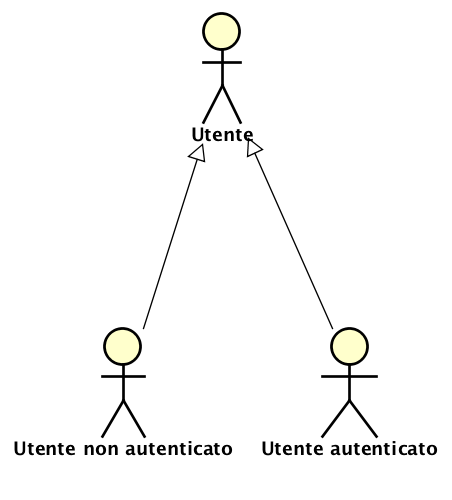
\includegraphics[scale=1]{../immagini/attori.png}
\caption{Gerarchia attori}
\end{figure}

\newpage
\subsection{UC 1 - Sistema Quizzipedia}

\begin{figure}[h!]
\centering
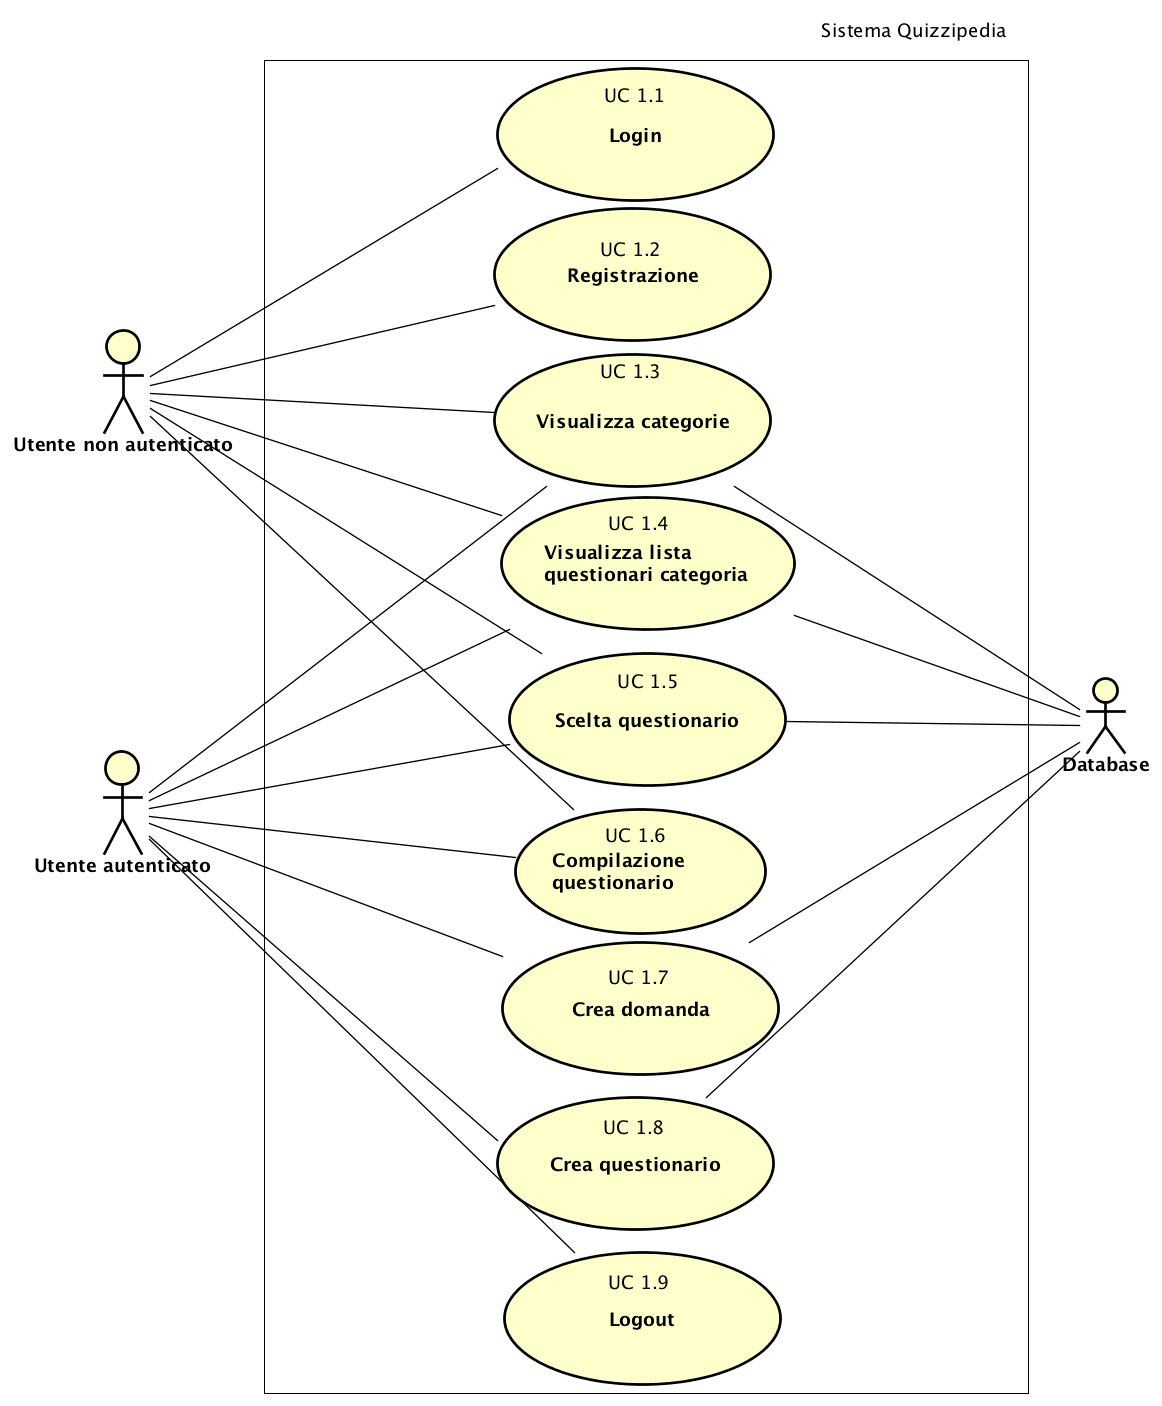
\includegraphics[scale=0.5]{../immagini/UC1.png}
\caption{UC 1 - Sistema Quizzipedia}
\end{figure}
\ \\
\textbf{Attori Principali:} \textit{utente non autenticato, utente autenticato}
\\
\textbf{Attori Secondari:} Database.\\
\\
\textbf{Descrizione:} il caso d'uso descrive le operazioni che i vari tipi di utenti possono effettuare all'interno del sistema.\\
\\
\textbf{Precondizioni:} l'utente è entrato in Quizzipedia.\\
\\
\textbf{Postcondizioni:} l'utente ha eseguito una delle operazioni possibili all'interno del sistema.\\
\\
\textbf{Scenari:}
\begin{itemize}
\item \textbf{Principale: } l'utente esegue una delle operazioni a lui permesse. Queste comprendono la visualizzazione delle categorie (UC 1.3) con successiva visualizzazione della lista dei questionari della categoria scelta (UC 1.4), la scelta di un questionario (UC 1.5) e la compilazione del questionario scelto (UC 1.6). Inoltre un utente non autenticato può registrarsi (UC 1.2) se non l'ha ancora fatto o accede con il proprio account (UC 1.1). Un utente autenticato può invece creare nuove domande (UC 1.7) o questionari (UC 1.8) oppure uscire dal sistema facendo il logout (UC 1.9).
\item \textbf{Alternativo: } l'utente esce da Quizzipedia.
\end{itemize}
\newpage
\subsection{UC 1.1 - Login}
\begin{figure}[h!]
\centering
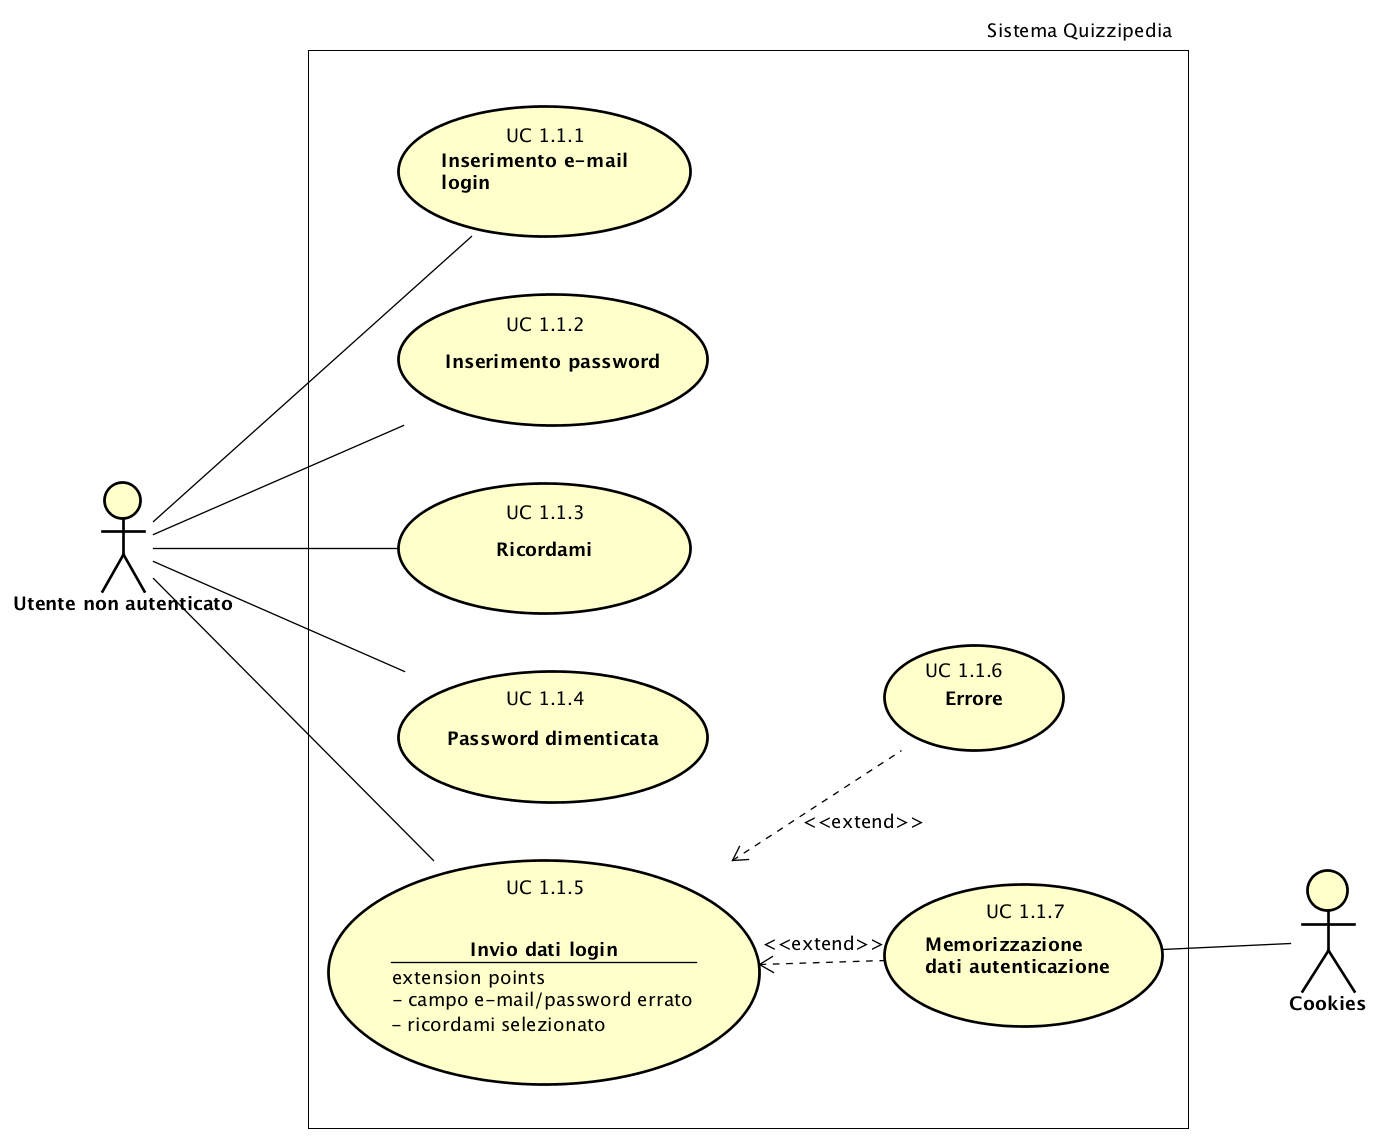
\includegraphics[scale=0.4]{../immagini/UC1_1.png}
\caption{UC 1.1 - Login}
\end{figure}

\ \\
\textbf{Attori Principali:} \textit{utente non autenticato}
\\
\textbf{Attori Secondari:} Cookies.\\
\\
\textbf{Descrizione:} il caso d'uso descrive le operazioni che l'utente non autenticato può fare per effettuare l'accesso al sistema.\\
\\
\textbf{Precondizioni:} il sistema può ricevere richieste di accesso da parte dell'utente non autenticato.\\
\\
\textbf{Postcondizioni:} il sistema ha riconosciuto i dati immessi dall'utente che ora è autenticato.\\
\\
\textbf{Scenari:}
\begin{itemize}
\item \textbf{Principale: } l'utente inserisce i dati di accesso per effettuare il login al sistema (UC 1.1.1 e 1.1.2). Ha la possibilità di selezionare inoltre l'opzione \textit{Ricordami} (UC 1.1.3) per mantenere in memoria la sua e-mail. Nel caso avesse dimenticato la password può accedere ad un form di recupero della stessa (UC 1.1.4). 
\item \textbf{Alternativo: } l'utente inserisce i dati di accesso per effettuare il login al sistema ma non sono corretti e il sistema avverte l'utente fornendogli la possibilità di ricompilare i campi. L'utente resta non autenticato.
\end{itemize}

\vspace{6 mm}

\subsubsection{UC 1.1.1 - Inserimento e-mail login}
\ \\
\textbf{Attori principali:} \textit{utente non autenticato}.\\
\\
\textbf{Descrizione:} il caso d'uso descrive l'inserimento da parte dell'utente della propria e-mail di riferimento per il login. \\
\\
\textbf{Precondizioni:} il sistema è nella schermata di login e offre un campo per l'inserimento della e-mail di login.\\
\\
\textbf{Postcondizioni:} l'utente ha digitato la sua e-mail. \\
\\
\textbf{Scenari:}
\begin{itemize}
\item \textbf{Principale:} l'utente inserisce la propria e-mail.
\end{itemize}

\vspace{6 mm}

\subsubsection{UC 1.1.2 - Inserimento password}
\ \\
\textbf{Attori principali:} \textit{utente non autenticato}.\\
\\
\textbf{Descrizione:} il caso d'uso descrive l'inserimento da parte dell'utente della propria password per il login. \\
\\
\textbf{Precondizioni:} il sistema è nella schermata di login e offre un campo per l'inserimento della password.\\
\\
\textbf{Postcondizioni:} l'utente ha digitato la sua password. \\
\\
\textbf{Scenari:}
\begin{itemize}
\item \textbf{Principale:} l'utente inserisce la propria password.
\end{itemize}

\vspace{6 mm}

\subsubsection{UC 1.1.3 - Ricordami}
\ \\
\textbf{Attori principali:} \textit{utente non autenticato}.\\
\\
\textbf{Descrizione:} il caso d'uso descrive la possibilità che ha l'utente di utilizzare l'opzione \textit{ricordami} per mantenere in memoria la propria e-mail. \\
\\
\textbf{Precondizioni:} il sistema è nella schermata di login e offre un'opzione \textit{ricordami}.\\
\\
\textbf{Postcondizioni:} l'utente ha selezionato l'opzione \textit{ricordami}. \\
\\
\textbf{Scenari:}
\begin{itemize}
\item \textbf{Principale:} l'utente seleziona l'opzione \textit{ricordami}.
\end{itemize}

\newpage

\subsubsection{UC 1.1.4 - Password dimenticata}
\begin{figure}[h!]
\centering
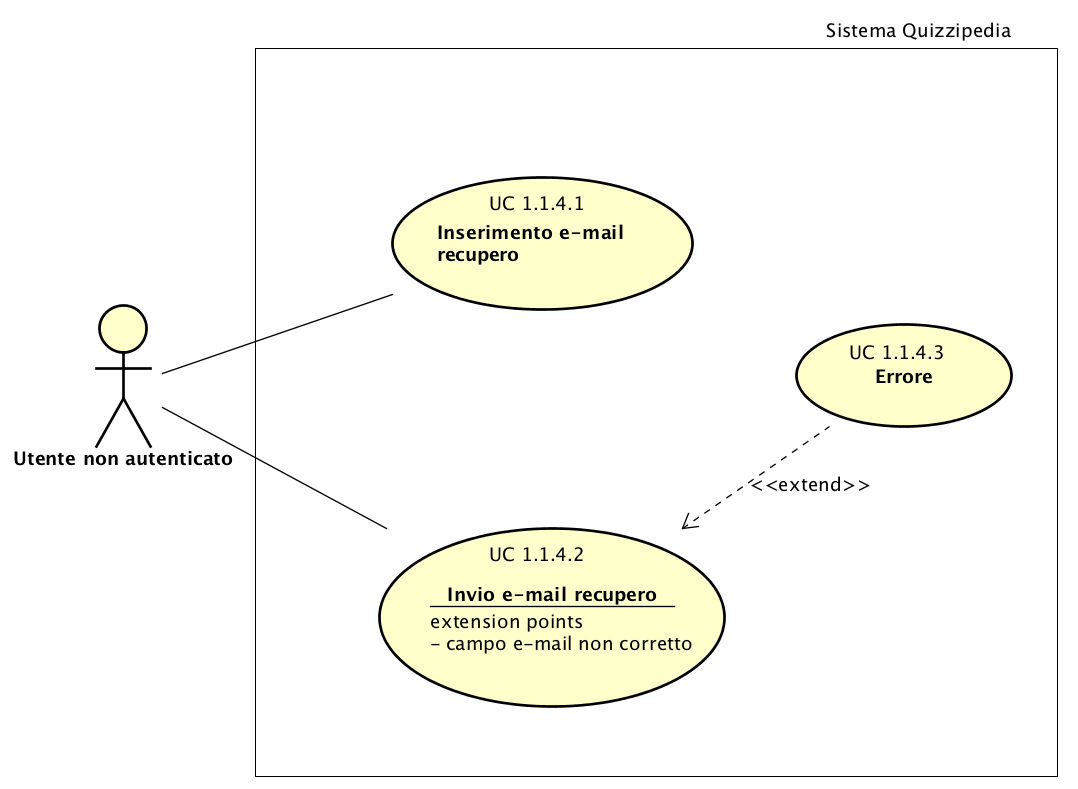
\includegraphics[scale=0.5]{../immagini/UC1_1_4.png}
\caption{UC 1.1.4 - Password dimenticata}
\end{figure}
\ \\
\textbf{Attori principali:} \textit{utente non autenticato}.\\
\\
\textbf{Descrizione:} il caso d'uso descrive la possibilità che ha l'utente di recuperare la propria password nel caso l'avesse dimenticata. Selezionando questa opzione l'utente può quindi utilizzare il form di recupero password compilando l'apposito campo con la sua e-mail di riferimento per il login (UC 1.1.4.1). \\
\\
\textbf{Precondizioni:} il sistema è nella schermata di login e fornisce un link per il recupero password.\\
\\
\textbf{Postcondizioni:} l'utente ha compilato il form di recupero password e il sistema ha provveduto ad inviare una e-mail all'indirizzo indicato dall'utente . \\
\\
\textbf{Scenari:}
\begin{itemize}
\item \textbf{Principale:} l'utente seleziona l'opzione \textit{Password dimenticata}.
\item \textbf{Alternativo:} l'utente non seleziona l'opzione \textit{Password dimenticata}.
\end{itemize}

\vspace{6 mm}

\subsubsection{UC 1.1.4.1 - Inserimento e-mail recupero}
\ \\
\textbf{Attori principali:} \textit{utente non autenticato}.\\
\\
\textbf{Descrizione:} il caso d'uso descrive l'inserimento da parte dell'utente della sua e-mail di riferimento all'interno del form di recupero password. \\
\\
\textbf{Precondizioni:} l'utente ha selezionato l'opzione \textit{Password dimenticata} (UC 1.1.4) e il sistema visualizza il form per il recupero. \\
\\
\textbf{Postcondizioni:} l'utente ha digitato la propria e-mail. \\
\\
\textbf{Scenari:}
\begin{itemize}
\item \textbf{Principale:} l'utente inserisce la propria e-mail.
\end{itemize}

\vspace{6 mm}

\subsubsection{UC 1.1.4.2 - Invio e-mail recupero}
\ \\
\textbf{Attori principali:} \textit{utente non autenticato}.\\
\\
\textbf{Descrizione:} il caso d'uso descrive l'invio al sistema da parte dell'utente della sua e-mail (UC 1.1.4.1).\\
\\
\textbf{Precondizioni:} l'utente ha digitato la propria mail nell'apposito campo (UC 1.1.4.1). L'utente deve essere non autenticato.\\
\\
\textbf{Postcondizioni:} Il sistema ha provveduto ad inviare una e-mail per comunicare la password. \\
\\
\textbf{Scenari:}
\begin{itemize}
\item \textbf{Principale:} l'utente fa mandare dal sistema una mail con la password dimenticata al proprio indirizzo e-mail.
\end{itemize}
\textbf{Extension points:}
\begin{itemize}
\item \textbf{e-mail non registrata:} il sistema avverte l'utente che l'e-mail inserita non è registrata.
\end{itemize}
\ \\
\subsubsection{UC 1.1.5 - Invio dati login}
\ \\
\textbf{Attori principali:} \textit{utente non autenticato}.\\
\\
\textbf{Attori Secondari:} cookies.\\
\\
\textbf{Descrizione:} il caso d'uso descrive l'invio da parte dell'utente dei dati di compilazione del form di login. \\
\\
\textbf{Precondizioni:} il sistema è nella schermata di login e offre un form per l'inserimento dei dati.\\
\\
\textbf{Postcondizioni:} l'utente è ora autenticato. Nel caso in cui l'opzione \textit{Ricordami} fosse stata selezionata, l'e-mail viene memorizzata come un cookie. \\
\\
\textbf{Scenari:}
\begin{itemize}
\item \textbf{Principale:} l'utente invia i dati tramite il form di login. I dati sono corretti e l'utente viene autenticato. Se l'opzione \textit{Ricordami} è stata selezionata l'e-mail viene memorizzata nei cookies.
\item \textbf{Alternativo:} l'utente invia i dati tramite il form di login ma i dati non sono corretti, viene avvisato l'utente e si invita a riprovare.
\end{itemize}
\textbf{Extension points:}
\begin{itemize}
\item \textbf{combinazione e-mail/password non corretta:} il sistema avverte l'utente che la combinazione e-mail password non è corretta. 

\end{itemize}

\newpage

\subsection{UC 1.2 - Registrazione}

\begin{figure}[h!]
\centering
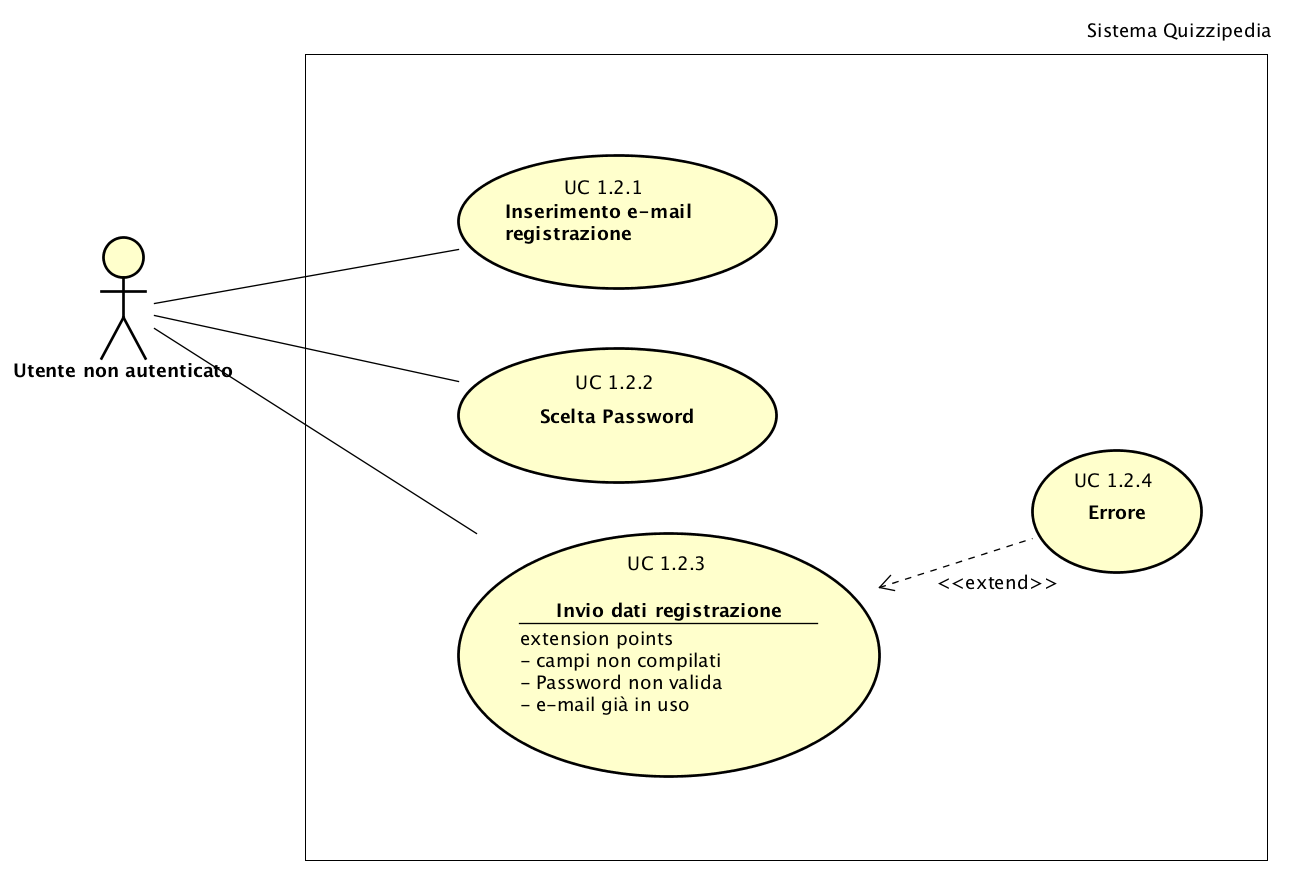
\includegraphics[scale=0.4]{../immagini/UC1_2.png}
\caption{UC 1.2 - Registrazione}
\end{figure}
\ \\
\textbf{Attori principali:} \textit{utente non autenticato}.\\
\\
\textbf{Descrizione:} il caso d'uso descrive le operazioni che un utente non autenticato può fare per effettuare la registrazione al sistema. \\
\\
\textbf{Precondizioni:} il sistema è nella condizione di poter ricevere dati di input relativi alla registrazione di un nuovo utente.\\
\\
\textbf{Postcondizioni:} il nuovo utente è ora registrato nel sistema. \\
\\
\textbf{Scenari:}
\begin{itemize}
\item \textbf{Principale:} l'utente compila i campi necessari alla registrazione (UC 1.2.1 e 1.2.2) e invia i dati al sistema (UC 1.2.3).

\end{itemize}
\vspace{6 mm}
\subsubsection{UC 1.2.1 - Inserimento e-mail registrazione}

\textbf{Attori principali:} \textit{utente non autenticato}.\\
\\
\textbf{Descrizione:} il caso d'uso descrive l'inserimento da parte dell'utente della propria e-mail.
\\
\textbf{Precondizioni:} il sistema è nella schermata di registrazione e fornisce all'utente il campo da compilare con la propria e-mail.\\
\\
\textbf{Postcondizioni:} l'utente ha digitato la propria e-mail nell'apposito campo. \\
\\
\textbf{Scenari:}
\begin{itemize}
\item \textbf{Principale:} l'utente compila il campo e-mail.

\end{itemize}
\vspace{6 mm}
\subsubsection{UC 1.2.2 - Scelta password}

\textbf{Attori principali:} \textit{utente non autenticato}.\\
\\
\textbf{Descrizione:} il caso d'uso descrive l'inserimento da parte dell'utente della password scelta.
\\
\textbf{Precondizioni:} il sistema è nella schermata di registrazione e fornisce all'utente il campo da compilare con la propria password.\\
\\
\textbf{Postcondizioni:} l'utente ha digitato la password scelta nell'apposito campo. \\
\\
\textbf{Scenari:}
\begin{itemize}
\item \textbf{Principale:} l'utente compila il campo password.

\end{itemize}

\vspace{6 mm}

\subsubsection{UC 1.2.3 - Invio dati registrazione}

\textbf{Attori principali:} \textit{utente non autenticato}.\\
\\
\textbf{Descrizione:} il caso d'uso descrive l'invio dei dati di registrazione appositamente compilati (UC 1.2.1 e 1.2.2).\\
\\
\textbf{Precondizioni:} il sistema è nella condizione di poter registrare un nuovo utente.\\
\\
\textbf{Postcondizioni:} l'utente è ora registrato. Inoltre viene effettuato in automatico il login, l'utente è quindi anche autenticato.\\
\\
\textbf{Scenari:}
\begin{itemize}
\item \textbf{Principale:} i dati inseriti (UC 1.2.1 e 1.2.2) vengono inviati al sistema di autenticazione che registra l'account.
\item \textbf{Alternativo:} i dati inseriti (UC 1.2.1 e 1.2.2) non risultano corretti, l'utente è invitato a ricompilare i campi.\\ 
\end{itemize}
\
\textbf{Extension points:}
\begin{itemize}
\item \textbf{campi non compilati:} il sistema avverte l'utente che alcuni o tutti i campi non sono stati compilati. 
\item \textbf{password non valida:} il sistema avverte l'utente che la password scelta (UC 1.2.2) non è conforme al formato indicato.
\item \textbf{e-mail già in uso:} il sistema avverte l'utente che l'e-mail inserita (UC 1.2.1) è già in uso.
\end{itemize}

\subsection{UC 1.3 - Visualizza categorie}

\textbf{Attori principali:} \textit{utente}.\\
\\
\textbf{Attori secondari:} \textit{database}.\\
\\
\textbf{Descrizione:} il caso d'uso descrive come un utente possa visualizzare le categorie di questionari nel database. \\
\\
\textbf{Precondizioni:} la pagina corrente ha un link alla sezione \textit{Categorie}. \\
\\
\textbf{Postcondizioni:} l'utente è ora nella sezione \textit{Categorie} nella quale c'è un elenco delle categorie di questionari presenti nel database. \\
\\
\textbf{Scenari:}
\begin{itemize}
\item \textbf{Principale:} l'utente clicca sul link ed entra nella sezione \textit{Categorie}.

\end{itemize}

\subsection{UC 1.4 - Visualizza lista questionari categoria}

\textbf{Attori principali:} \textit{utente}.\\
\\
\textbf{Attori secondari:} \textit{database}.\\
\\
\textbf{Descrizione:} il caso d'uso descrive come un utente possa visualizzare i questionari presenti nel database della categoria selezionata (UC 1.3). \\
\\
\textbf{Precondizioni:} l'utente è nella sezione \textit{Categorie}. \\
\\
\textbf{Postcondizioni:} l'utente visualizza un elenco dei questionari della categoria scelta presenti nel database. \\
\\
\textbf{Scenari:}
\begin{itemize}
\item \textbf{Principale:} l'utente seleziona una categoria dall'elenco e viene visualizzata la lista dei questionari della categoria scelta presenti nel database.

\end{itemize}

\subsection{UC 1.5 - Scelta questionario}

\textbf{Attori principali:} \textit{utente}.\\
\\
\textbf{Attori secondari:} \textit{database}.\\
\\
\textbf{Descrizione:} il caso d'uso descrive la scelta di un questionario da parte dell'utente. \\
\\
\textbf{Precondizioni:} l'utente visualizza un elenco di questionari. \\
\\
\textbf{Postcondizioni:} l'utente visualizza il questionario scelto e può ora procedere alla sua compilazione. \\
\\
\textbf{Scenari:}
\begin{itemize}
\item \textbf{Principale:} l'utente seleziona un questionario dall'elenco e questo viene letto dal database e visualizzato per la compilazione.

\end{itemize}

\newpage

\subsection{UC 1.6 - Compilazione questionario}

\begin{figure}[h!]
\centering
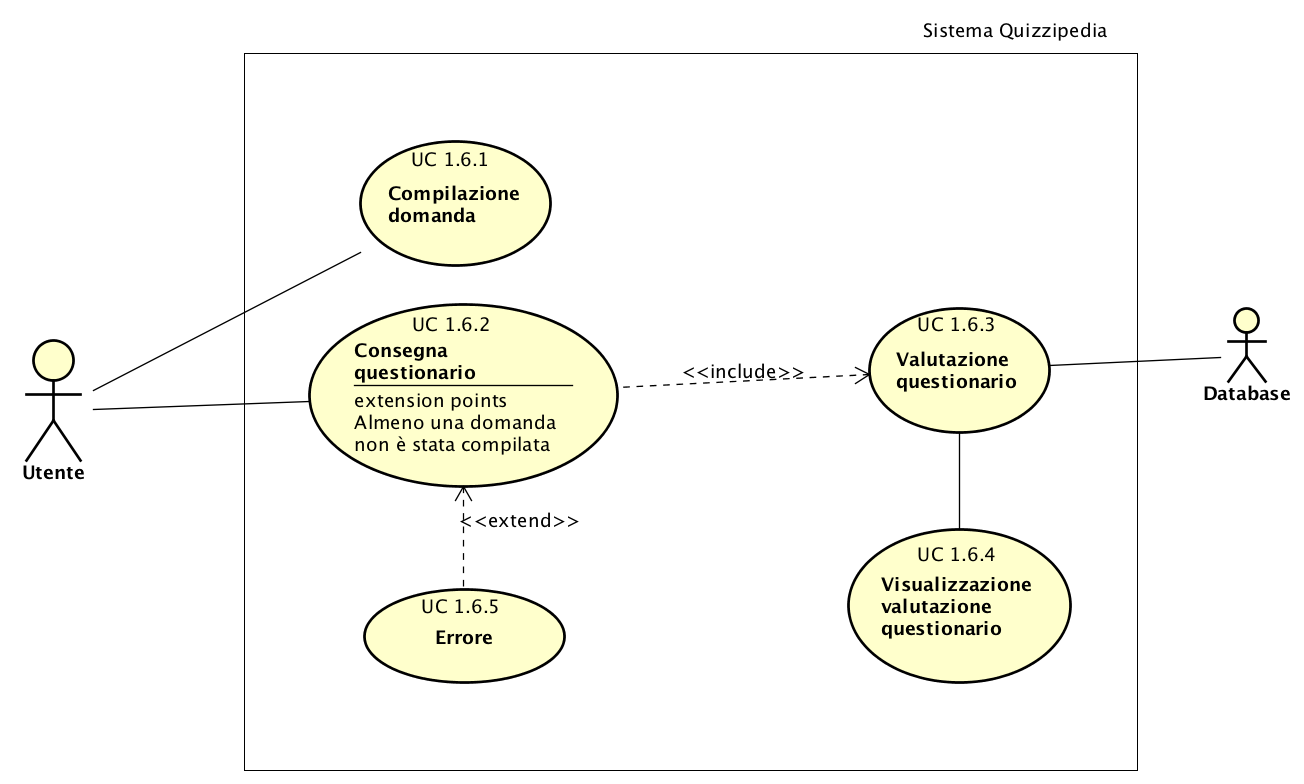
\includegraphics[scale=0.4]{../immagini/UC1_6.png}
\caption{UC 1.6 - Compilazione questionario}
\end{figure}
\ \\
\textbf{Attori principali:} \textit{utente}.\\
\ \\
\textbf{Attori secondari:} \textit{database}.\\
\\
\textbf{Descrizione:} il caso d'uso descrive la compilazione di un questionario scelto. \\
\\
\textbf{Precondizioni:} il sistema è nella schermata di visualizzazione di un questionario.\\
\\
\textbf{Postcondizioni:} l'utente ha compilato il questionario e vengono visualizzati i risultati. \\
\\
\textbf{Scenari:}
\begin{itemize}
\item \textbf{Principale:} l'utente risponde alle domande e riceve una valutazione sul questionario compilato.
\item \textbf{Alternativo:} l'utente rinuncia alla compilazione e torna indietro.\\ 
\end{itemize}
\vspace{6 mm}
\subsubsection{UC 1.6.1 - Compilazione domanda}

\textbf{Attori principali:} \textit{utente}.\\
\\
\textbf{Descrizione:} il caso d'uso descrive la risposta di una domanda da parte dell'utente. \\
\\
\textbf{Precondizioni:} il sistema visualizza la domanda e le eventuali alternative di risposta o permette l'inserimento di quest'ultima.\\
\\
\textbf{Postcondizioni:} l'utente ha risposto alla domanda. \\
\\
\textbf{Scenari:}
\begin{itemize}
\item \textbf{Principale:} l'utente inserisce una risposta alla domanda.
\item \textbf{Alternativo:} l'utente sceglie una delle possibili risposte alla domanda.\\ 
\end{itemize}
\vspace{6 mm}
\subsubsection{UC 1.6.2 - Consegna questionario}

\textbf{Attori principali:} \textit{utente}.\\
\\
\textbf{Descrizione:} il caso d'uso descrive la consegna del questionario compilato. \\
\\
\textbf{Precondizioni:} il sistema è nella schermata di compilazione di un questionario e l'utente lo conferma cliccando il comando di consegna.\\
\\
\textbf{Postcondizioni:} l'utente ha consegnato il questionario compilato. \\
\\
\textbf{Scenari:}
\begin{itemize}
\item \textbf{Principale:} l'utente conferma il questionario cliccando il comando di consegna.
\item \textbf{Alternativo:} l'utente non consegna il questionario e continua a compilarlo. \\
\item \textbf{Alternativo:} l'utente non consegna il questionario ed esce dalla compilazione.\\ 
\end{itemize}
\
\textbf{Extension points:}
\begin{itemize}
\item \textbf{domanda non compilata:} il sistema avverte l'utente che almeno una domanda non è stata compilata.
\end{itemize}
\vspace{6 mm}
\subsubsection{UC 1.6.3 - Valutazione questionario}

\textbf{Attori principali:} \textit{utente}.\\
\ \\
\textbf{Attori secondari:} \textit{Database}.\\
\\
\textbf{Descrizione:} il caso d'uso descrive la valutazione di un questionario. \\
\\
\textbf{Precondizioni:} l'utente ha compilato un questionario e lo ha consegnato.\\
\\
\textbf{Postcondizioni:} le risposte inserite vengono confrontate con quelle corrette e si ottiene una valutazione. \\
\\
\textbf{Scenari:}
\begin{itemize}
\item \textbf{Principale:} il sistema valuta le risposte del questionario consegnato.
\end{itemize}
\vspace{6 mm}
\subsubsection{UC 1.6.4 - Visualizzazione valutazione questionario}

\textbf{Attori principali:} \textit{utente}.\\
\\
\textbf{Descrizione:} il caso d'uso descrive la visualizzazione della valutazione di un questionario. \\
\\
\textbf{Precondizioni:} l'utente ha consegnato un questionario e questo è stato valutato.\\
\\
\textbf{Postcondizioni:} l'utente visualizza i risultati ottenuti. \\
\\
\textbf{Scenari:}
\begin{itemize}
\item \textbf{Principale:} vengono visualizzati i risultati del questionario consegnato e valutato.
\end{itemize}

\newpage

\subsection{UC 1.7 - Crea domanda}

\begin{figure}[h!]
\centering
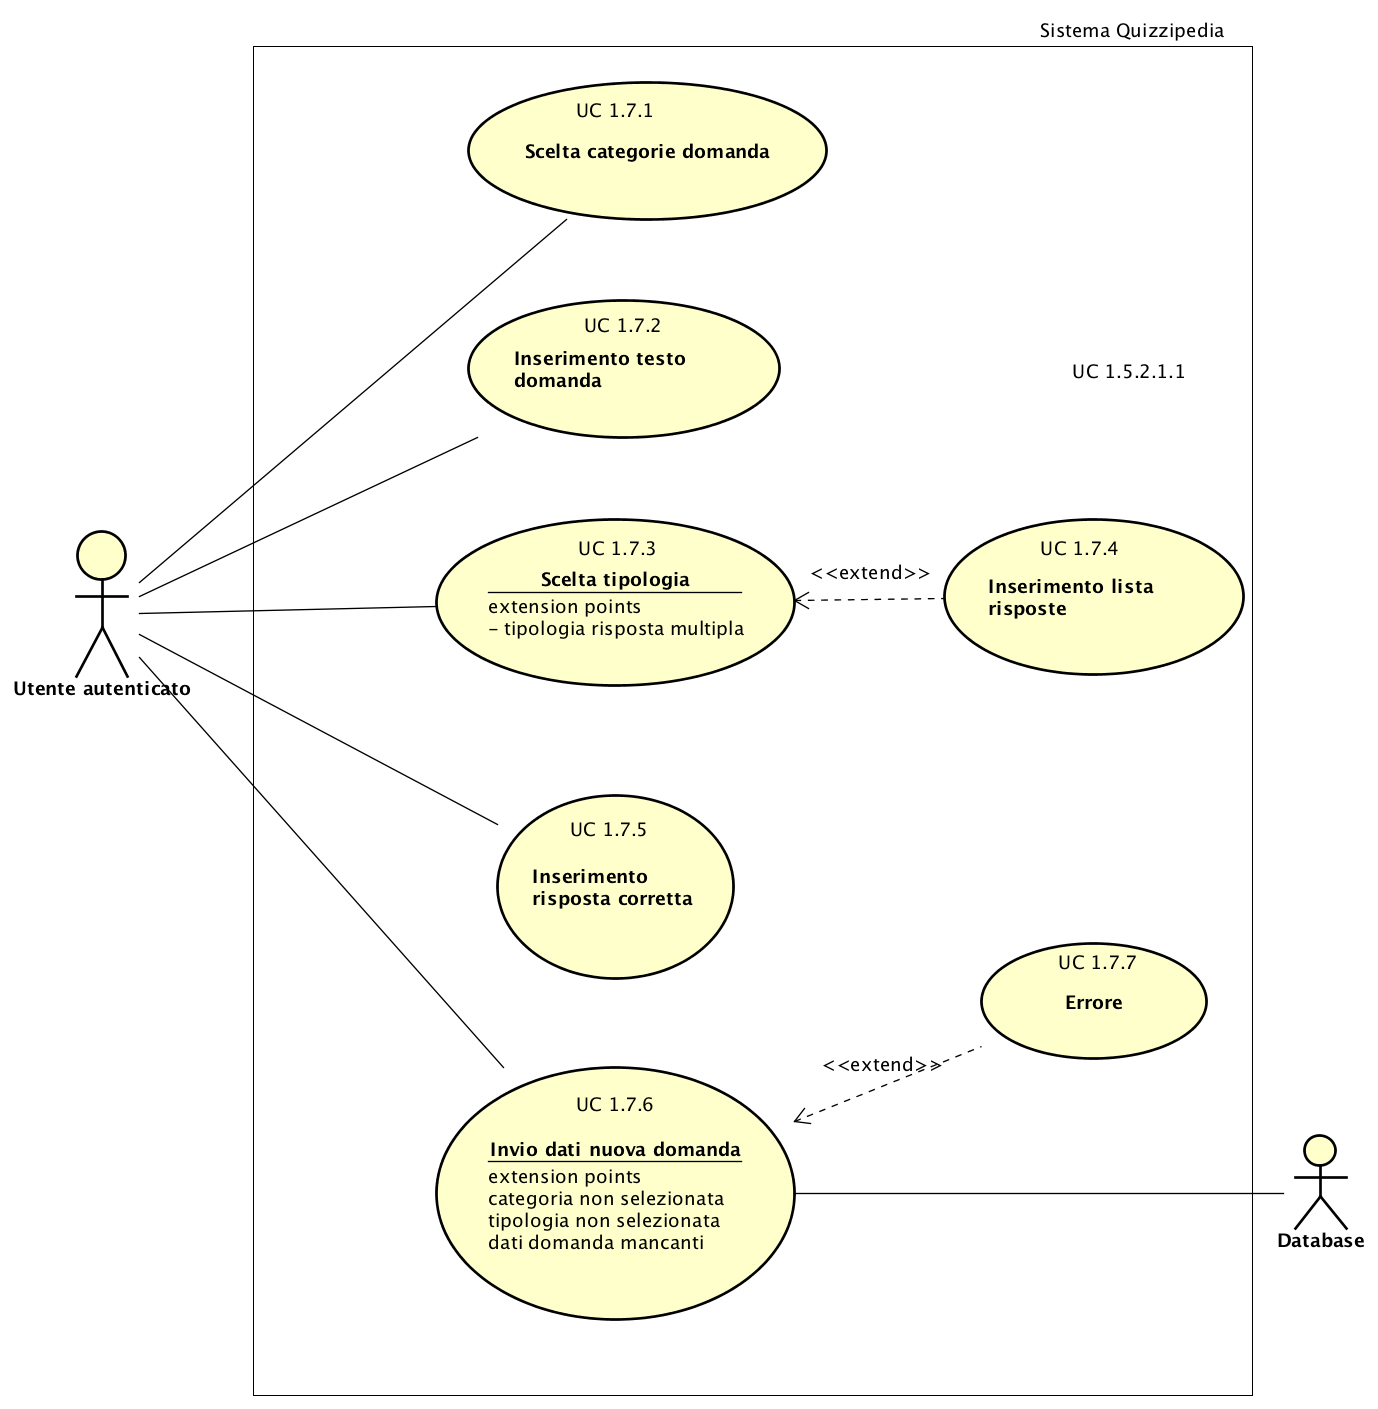
\includegraphics[scale=0.4]{../immagini/UC1_7.png}
\caption{UC 1.7 - Crea Domanda}
\end{figure}
\ \\
\textbf{Attori principali:} \textit{utente autenticato}.\\
\\
\textbf{Attori secondari:} \textit{database}.\\
\\
\textbf{Descrizione:} il caso d'uso descrive la creazione di una nuova domanda. \\
\\
\textbf{Precondizioni:} l'utente è autenticato e la pagina corrente fornisce un link alla sezione di creazione di una domanda.\\
\\
\textbf{Postcondizioni:} l'utente ha creato una nuova domanda, che viene aggiunta al database. \\
\\
\textbf{Scenari:}
\begin{itemize}
\item \textbf{Principale:} l'utente inserisce i dati e crea una nuova domanda, che viene aggiunta al database.
\item \textbf{Alternativo:} l'utente rinuncia alla creazione della domanda e torna indietro.\\ 
\end{itemize}
\vspace{6 mm}
\subsubsection{UC 1.7.1 - Scelta categorie domanda}

\textbf{Attori principali:} \textit{utente autenticato}.\\
\\
\textbf{Descrizione:} il caso d'uso descrive la scelta di una o più categorie che la domanda riguarda. \\
\\
\textbf{Precondizioni:} il sistema è nella schermata di creazione di una nuova domanda e fornisce all'utente più scelte della categoria della domanda.\\
\\
\textbf{Postcondizioni:} l'utente ha scelto una o più categorie per la nuova domanda. \\
\\
\textbf{Scenari:}
\begin{itemize}
\item \textbf{Principale:} l'utente sceglie una o più categorie.
\end{itemize}
\vspace{6 mm}
\subsubsection{UC 1.7.2 - Inserimento testo domanda}

\textbf{Attori principali:} \textit{utente autenticato}.\\
\\
\textbf{Descrizione:} il caso d'uso descrive l'inserimento del testo della nuova domanda. \\
\\
\textbf{Precondizioni:} il sistema è nella schermata di creazione di una nuova domanda e fornisce all'utente un'area da compilare con il testo della domanda.\\
\\
\textbf{Postcondizioni:} l'utente ha inserito il testo della nuova domanda. \\
\\
\textbf{Scenari:}
\begin{itemize}
\item \textbf{Principale:} l'utente inserisce il testo della domanda.
\end{itemize}
\vspace{6 mm}
\subsubsection{UC 1.7.3 - Scelta tipologia domanda}

\textbf{Attori principali:} \textit{utente autenticato}.\\
\\
\textbf{Descrizione:} il caso d'uso descrive la scelta della tipologia della nuova domanda. \\
\\
\textbf{Precondizioni:} il sistema è nella schermata di creazione di una nuova domanda e fornisce all'utente una scelta della tipologia della domanda.\\
\\
\textbf{Postcondizioni:} l'utente ha scelto le categorie della nuova domanda. \\
\\
\textbf{Scenari:}
\begin{itemize}
\item \textbf{Principale:} l'utente sceglie la tipologia della domanda.
\end{itemize}
\
\textbf{Extension points:}
\begin{itemize}
\item \textbf{tipologia risposta multipla:} il sistema richiede la lista delle alternative di risposta.
\end{itemize}
\vspace{6 mm}
\subsubsection{UC 1.7.5 - Inserimento risposta corretta}

\textbf{Attori principali:} \textit{utente autenticato}.\\
\\
\textbf{Descrizione:} il caso d'uso descrive l'inserimento o la scelta della risposta corretta. \\
\\
\textbf{Precondizioni:} il sistema è nella schermata di creazione di una nuova domanda e fornisce all'utente un campo da compilare oppure una scelta della risposta corretta alla domanda.\\
\\
\textbf{Postcondizioni:} l'utente ha inserito o scelto la risposta corretta alla domanda. \\
\\
\textbf{Scenari:}
\begin{itemize}
\item \textbf{Principale:} l'utente inserisce la risposta corretta alla domanda.
\item \textbf{Alternativo:} l'utente sceglie la risposta corretta alla domanda tra quelle possibili inserite precedentemente. Questa opzione è disponibile solo se la domanda è di tipo scelta multipla.
\end{itemize}
\vspace{6 mm}
\subsubsection{UC 1.7.6 - Invio dati nuova domanda}

\textbf{Attori principali:} \textit{utente autenticato}.\\
\\
\textbf{Attori secondari:} \textit{database}.\\
\\
\textbf{Descrizione:} il caso d'uso descrive la conferma e l'invio dei dati della nuova domanda. \\
\\
\textbf{Precondizioni:} il sistema è nella schermata di creazione di una nuova domanda e fornisce all'utente un bottone di conferma e invio dati della domanda.\\
\\
\textbf{Postcondizioni:} l'utente ha creato la nuova domanda, che è stata inserita nel database. \\
\\
\newpage
\textbf{Scenari:}
\begin{itemize}
\item \textbf{Principale:} l'utente conferma e invia i dati relativi alla nuova domanda e questa viene aggiunta al database.
\end{itemize}
\
\textbf{Extension points:}
\begin{itemize}
\item \textbf{categoria non selezionata:} il sistema avvisa l'utente che non è stata selezionata nessuna categoria.
\item \textbf{tipologia non selezionata:} il sistema avvisa l'utente che non è stata selezionata nessuna tipologia di domanda.
\item \textbf{dati domanda mancanti:} il sistema avvisa l'utente che non sono stati inseriti dati essenziali per la creazione della domanda.
\end{itemize}

\newpage

\subsection{UC 1.8 - Crea questionario}

\begin{figure}[h!]
\centering
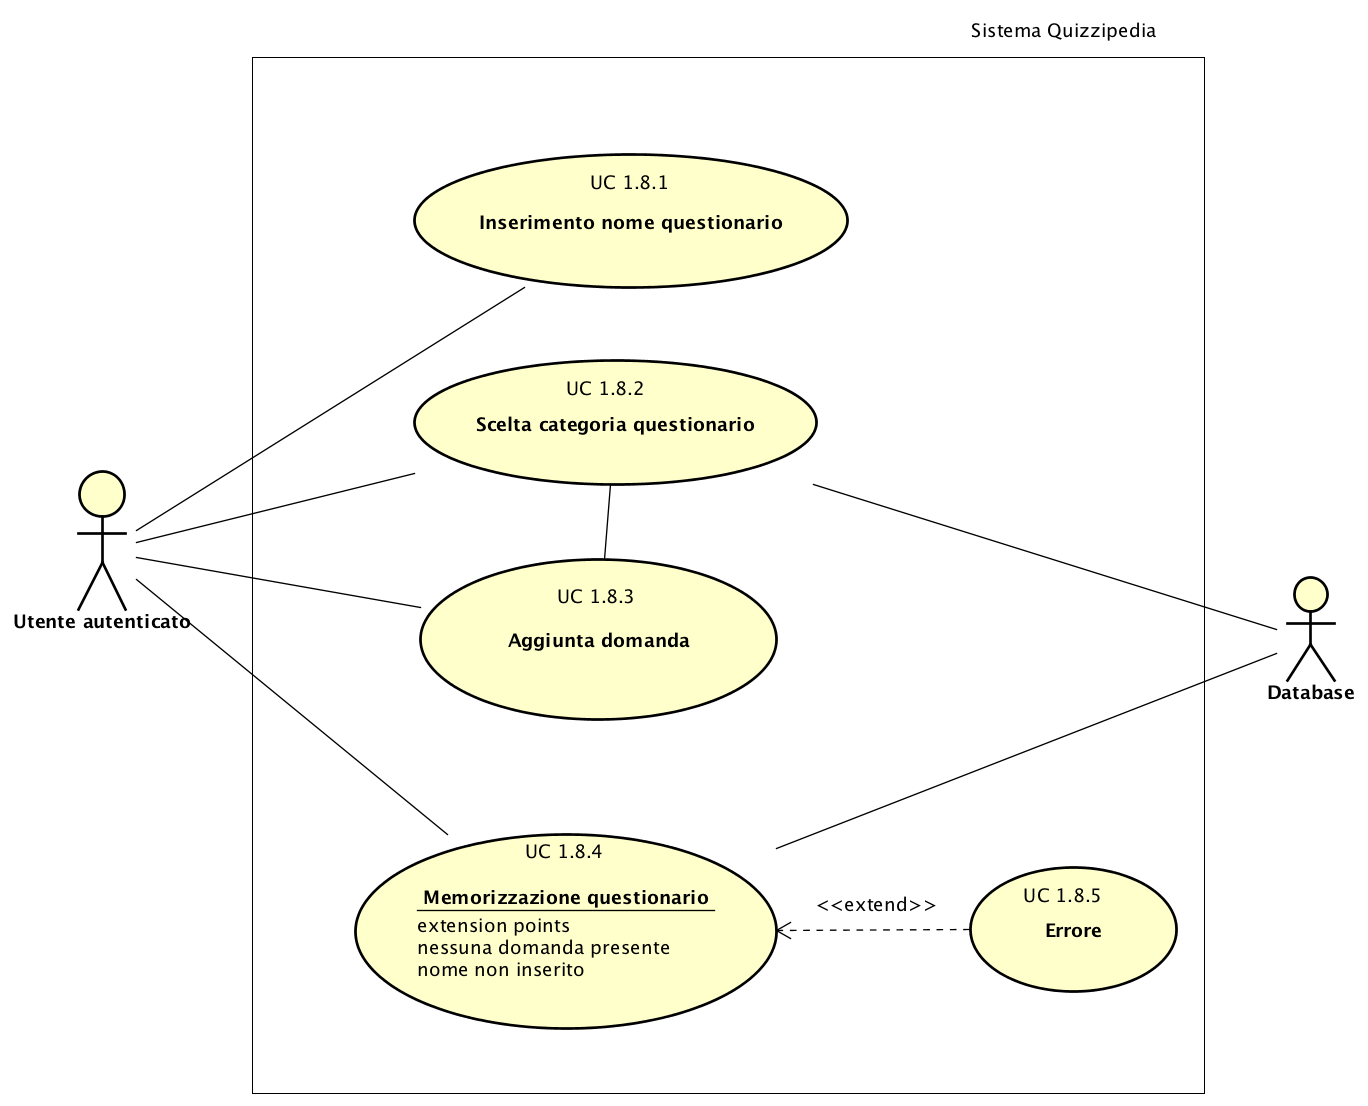
\includegraphics[scale=0.4]{../immagini/UC1_8.png}
\caption{UC 1.8 - Crea questionario}
\end{figure}
\ \\
\textbf{Attori principali:} \textit{utente autenticato}.\\
\\
\textbf{Attori secondari:} \textit{database}.\\
\\
\textbf{Descrizione:} il caso d'uso descrive la creazione di un nuovo questionario. \\
\\
\textbf{Precondizioni:} l'utente è autenticato e la pagina corrente fornisce un link alla sezione di creazione di un questionario.\\
\\
\textbf{Postcondizioni:} l'utente ha creato un nuovo questionario, che viene aggiunto al database. \\
\\
\textbf{Scenari:}
\begin{itemize}
\item \textbf{Principale:} l'utente inserisce i dati e crea un nuovo questionario, che viene aggiunto al database.
\item \textbf{Alternativo:} l'utente rinuncia alla creazione del questionario e torna indietro.\\ 
\end{itemize}
\vspace{6 mm}
\subsubsection{UC 1.8.1 - Inserimento nome questionario}

\textbf{Attori principali:} \textit{utente autenticato}.\\
\\
\textbf{Descrizione:} il caso d'uso descrive l'inserimento del nome del nuovo questionario. \\
\\
\textbf{Precondizioni:} il sistema è nella schermata di creazione di un nuovo questionario e fornisce all'utente un campo da compilare con il nome del questionario.\\
\\
\textbf{Postcondizioni:} l'utente ha inserito il nome del nuovo questionario. \\
\\
\textbf{Scenari:}
\begin{itemize}
\item \textbf{Principale:} l'utente inserisce il nome del questionario.
\end{itemize}
\vspace{6 mm}
\subsubsection{UC 1.8.2 - Scelta categoria questionario}

\textbf{Attori principali:} \textit{utente autenticato}.\\
\\
\textbf{Attori secondari:} \textit{database}.\\
\\
\textbf{Descrizione:} il caso d'uso descrive la scelta della categoria del questionario. \\
\\
\textbf{Precondizioni:} il sistema è nella schermata di creazione di un nuovo questionario e fornisce all'utente una scelta per la categoria del questionario.\\
\\
\textbf{Postcondizioni:} l'utente ha scelto la categoria del questionario e viene visualizzata la lista di domande di quella categoria che possono essere inserite nel questionario. \\
\\
\textbf{Scenari:}
\begin{itemize}
\item \textbf{Principale:} l'utente sceglie la categoria del questionario. Successivamente viene visualizzata la lista delle domande della categoria selezionata che possono essere inserite nel questionario.
\end{itemize}
\vspace{6 mm}
\subsubsection{UC 1.8.3 - Aggiunta domanda}

\textbf{Attori principali:} \textit{utente autenticato}.\\
\\
\textbf{Descrizione:} il caso d'uso descrive aggiunta di una domanda di quelle proposte nel nuovo questionario. \\
\\
\textbf{Precondizioni:} il sistema è nella schermata di creazione di un nuovo questionario e fornisce all'utente una lista di domande che possono essere inserite nel questionario e un modo per aggiungerle.\\
\\
\textbf{Postcondizioni:} l'utente ha aggiunto una domanda al questionario. \\
\\
\newpage
\textbf{Scenari:}
\begin{itemize}
\item \textbf{Principale:} l'utente aggiunge una domanda al questionario.
\end{itemize}
\vspace{6 mm}
\subsubsection{UC 1.8.4 - Memorizzazione questionario}

\textbf{Attori principali:} \textit{utente autenticato}.\\
\\
\textbf{Attori secondari:} \textit{database}.\\
\\
\textbf{Descrizione:} il caso d'uso descrive la conferma e la memorizzazione del questionario. \\
\\
\textbf{Precondizioni:} il sistema è nella schermata di creazione di un nuovo questionario e fornisce all'utente un bottone di conferma di creazione del questionario.\\
\\
\textbf{Postcondizioni:} l'utente ha creato un nuovo questionario. \\
\\
\textbf{Scenari:}
\begin{itemize}
\item \textbf{Principale:} l'utente conferma e crea un nuovo questionario.
\end{itemize}
\
\textbf{Extension points:}
\begin{itemize}
\item \textbf{nessuna domanda presente:} il sistema avvisa l'utente che non è stata aggiunta nessuna domanda al questionario.
\item \textbf{nome non inserito:} il sistema avvisa l'utente che non è stato inserito il nome del questionario.
\end{itemize}

\subsection{UC 1.9 - Logout}

\textbf{Attori principali:} \textit{utente autenticato}.\\
\\
\textbf{Descrizione:} il caso d'uso descrive l'uscita dal sistema da parte di un utente autenticato. \\
\\
\textbf{Precondizioni:} l'utente è autenticato. \\
\\
\textbf{Postcondizioni:} l'utente non è più autenticato. \\
\\
\textbf{Scenari:}
\begin{itemize}
\item \textbf{Principale:} l'utente esce dal sistema passando da autenticato a non autenticato.

\end{itemize}
	
	\newpage
	\section{Requisiti}
		Di seguito vengono elencati i requisiti emersi in fase di analisi del capitolato e del problema.\\
		I requisiti sono presentati in maniera gerarchica affinché i sotto-requisiti specifichino ulteriori informazioni e dettagli rispetto al loro genitore.\\
		Per avere una migliore organizzazione dei requisiti questi vengono suddivisi in funzionali (F), QML (QML), di qualità (Q) e vincoli di sistema imposti dal capitolato (V).\\
		Dopo la categoria ogni codice identificativo è completato da un numero che mostra anche il livello e l'appartenenza della gerarchia sopra descritta.\\
		\subsection{Requisiti funzionali}
			\begin{longtable}{p{0.2\columnwidth}p{0.8\textwidth}}
			\caption{Requisiti funzionali} \\

ID & Descrizione \\
\midrule
\endfirsthead

ID & Descrizione \\
\midrule
\endhead

\multicolumn{2}{c}{\footnotesize\itshape\tablename~\thetable: Requisiti funzionali}
\endfoot

\multicolumn{2}{c}{\footnotesize\itshape\tablename~\thetable: Requisiti funzionali}
\endlastfoot
			
F 1 & Il sistema deve fornire la possibilità ad un utente non autenticato di registrarsi\\
\midrule
F 1.1 & La sezione dedicata alla registrazione deve permettere l'inserimento dei dati necessari\\
\midrule
F 1.1.1 & La sezione dedicata alla registrazione deve permettere l'inserimento di una e-mail\\
\midrule
F 1.1.2 & La sezione dedicata alla registrazione deve permettere l'inserimento di una password\\
\midrule
F 1.2 & La sezione dedicata alla registrazione deve permettere l'invio dei dati inseriti\\
\midrule
F 1.2.1 & Prima di inviare i dati viene effettuato un controllo su di essi\\
\midrule
F 1.2.1.1 & Se i dati non risultano corretti viene visualizzato un messaggio di errore\\
\midrule
F 1.2.1.2 & Se i dati non risultano corretti non vengono inviati\\
\midrule
F 1.2.2 & Quando dei dati corretti vengono inviati il sistema memorizza un nuovo account con essi\\
\midrule
F 1.2.3 & Quando viene creato un nuovo account con la procedura di registrazione viene automaticamente effettuato il login con quell'account\\
\midrule
F 2 & Il sistema deve fornire la possibilità ad un utente non autenticato di autenticarsi\\
\midrule
F 2.1 & La sezione dedicata all'autenticazione deve permettere l'inserimento dei dati necessari\\
\midrule
F 2.1.1 & La sezione dedicata all'autenticazione deve permettere l'inserimento di una e-mail\\
\midrule
F 2.1.2 & La sezione dedicata all'autenticazione deve permettere l'inserimento di una password\\
\midrule
F 2.2 & La sezione dedicata all'autenticazione deve fornire l'opzione ricordami\\
\midrule
F 2.3 & La sezione dedicata all'autenticazione deve permettere l'invio dei dati inseriti\\
\midrule
F 2.3.1 & Prima di inviare i dati viene effettuato un controllo su di essi\\
\midrule
F 2.3.1.1 & Se la combinazione e-mail/password non è registrata viene visualizzato un messaggio di errore\\
\midrule
F 2.3.2 & Se la combinazione e-mail/password è registrata l'utente viene autenticato\\
\midrule
F 2.3.3 & Se la combinazione e-mail/password è registrata e l'opzione ricordami è stata selezionata viene memorizzata l'e-mail con un cookie\\
\midrule
F 2.4 & La sezione dedicata all'autenticazione deve fornire una procedura di recupero password\\
\midrule
F 2.4.1 & La procedura di recupero password deve permettere l'inserimento della e-mail\\
\midrule
F 2.4.2 & La procedura di recupero password deve effettuare un controllo sulla e-mail inserita\\
\midrule
F 2.4.2.1 & Se la e-mail non risulta registrata viene visualizzato un messaggio di errore\\
\midrule
F 2.4.2.2 & Se la e-mail non risulta registrata non viene mandata una mail a quell'indirizzo\\
\midrule
F 2.4.3 & La procedura di recupero password deve mandare una mail all'indirizzo inserito con la password dimenticata\\
\midrule
F 3 & Il sistema deve fornire una sezione con un elenco delle categorie di questionari presenti nel database\\
\midrule
F 3.1 & Quando l'utente seleziona una categoria viene visualizzato un elenco dei questionari della categoria scelta presenti nel database\\
\midrule
F 4 & L'utente può scegliere un qualsiasi questionario cliccandoci sopra per compilarlo\\
\midrule
F 4.1 & Durante la compilazione del questionario un utente può navigare liberamente tra le domande che lo compongono\\
\midrule
F 4.2 & L'utente può rispondere alle domande\\
\midrule
F 4.2.1 & Se la domanda è di tipo vero o falso vengono fornite due opzioni: Vero e Falso\\
\midrule
F 4.2.2 & Se la domanda è a risposta multipla vengono fornita la lista di possibili risposte\\
\midrule
F 4.2.3 & Se la domanda richiede una risposta inserita dall'utente allora viene fornito un campo per l'inserimento della risposta\\
\midrule
F 4.3 & L'utente può cambiare la risposta di una domanda in qualsiasi momento prima della consegna del questionario\\
\midrule
F 4.4 & Le domande possono essere compilate in un ordine qualsiasi\\
\midrule
F 4.5 & L'utente può consegnare il questionario\\
\midrule
F 4.5.1 & Se alla consegna una o più domande non sono state compilate il sistema avverte l'utente di ciò\\
\midrule
F 4.5.2 & Quando un questionario viene confermato e consegnato vengono memorizzate nel database le risposte date\\
\midrule
F 4.5.3 & Quando un questionario viene confermato e consegnato viene valutato dal sistema\\
\midrule
F 4.5.3.1 & La valutazione del questionario viene visualizzata all'utente\\
\midrule
F 5 & Il sistema deve fornire la possibilità ad un utente autenticato di creare una nuova domanda\\
\midrule
F 5.1 & La sezione dedicata alla creazione di una domanda deve permettere l'inserimento dei dati necessari\\
\midrule
F 5.1.1 & La sezione dedicata alla creazione di una domanda deve permettere la scelta di una o più categorie\\
\midrule
F 5.1.2 & La sezione dedicata alla creazione di una domanda deve permettere l'inserimento del testo della domanda\\
\midrule
F 5.1.3 & La sezione dedicata alla creazione di una domanda deve permettere la scelta della tipologia della domanda\\
\midrule
F 5.1.3.1 & Nel caso in cui la tipologia scelta sia a risposta multipla la sezione dedicata alla creazione di una domanda deve permettere l'inserimento di due o più possibili risposte\\
\midrule
F 5.1.4 & La sezione dedicata alla creazione di una domanda deve permettere l'inserimento della risposta corretta\\
\midrule
F 5.2 & La sezione dedicata alla creazione di una domanda deve permettere l'invio dei dati inseriti\\
\midrule
F 5.2.1 & Prima di inviare i dati viene effettuato un controllo su di essi\\
\midrule
F 5.2.1.1 & Se i dati obbligatori non risultano inseriti viene visualizzato un messaggio di errore\\
\midrule
F 5.2.1.2 & Se i dati obbligatori non risultano inseriti nessun dato viene inviato\\
\midrule
F 5.2.2 & Quando dei dati che superano i controlli vengono inviati viene creata una nuova domanda con essi e inserita nel database\\
\midrule
F 5.2.2.1 & Se la creazione di una nuova domanda va a buon fine il sistema avvisa l'utente\\
\midrule
F 5.2.2.2 & Se la creazione di una nuova domanda non va a buon fine il sistema visualizza un messaggio di errore\\
\midrule
F 6 & Il sistema deve fornire la possibilità ad un utente autenticato di creare un nuovo questionario\\
\midrule
F 6.1 & La sezione dedicata alla creazione di un questionario deve permettere l'inserimento dei dati necessari\\
\midrule
F 6.1.1 & La sezione dedicata alla creazione di un questionario deve permettere l'inserimento del nome del questionario\\
\midrule
F 6.1.2 & La sezione dedicata alla creazione di un questionario deve permettere la scelta della categoria del questionario\\
\midrule
F 6.1.2.1 & Una volta scelta la categoria la sezione dedicata alla creazione di un questionario deve visualizzare la lista delle domande di quella categoria presenti nel database non ancora inserite nel questionario\\
\midrule
F 6.1.3 & La sezione dedicata alla creazione di un questionario deve permettere l'aggiunta di una domanda della lista di F 6.1.2.1 nel questionario\\
\midrule
F 6.1.4 & La sezione dedicata alla creazione di un questionario deve visualizzare la lista di domande già inserite nel questionario\\
\midrule
F 6.2 & La sezione dedicata alla creazione di una nuova domanda deve permettere l'invio dei dati inseriti\\
\midrule
F 6.2.1 & Prima di inviare i dati viene effettuato un controllo su di essi\\
\midrule
F 6.2.1.1 & Se i dati obbligatori non risultano inseriti viene visualizzato un messaggio di errore\\
\midrule
F 6.2.1.2 & Se i dati obbligatori non risultano inseriti nessun dato viene inviato\\
\midrule
F 6.2.2 & Quando dei dati che superano i controlli vengono inviati viene creato un nuovo questionario con essi e inserito nel database\\
\midrule
F 6.2.2.1 & Se la creazione di un nuovo questionario va a buon fine il sistema avvisa l'utente\\
\midrule
F 6.2.2.2 & Se la creazione di un nuovo questionario non va a buon fine il sistema visualizza un messaggio di errore\\
\midrule
F 7 & Il sistema deve fornire la possibilità ad un utente autenticato di uscire facendo il logout\\
			
			\end{longtable}
		\subsection{Requisiti QML}
			\begin{longtable}{p{0.2\columnwidth}p{0.8\textwidth}}
			\caption{Requisiti QML} \\

ID & Descrizione \\
\midrule
\endfirsthead

ID & Descrizione \\
\midrule
\endhead

\multicolumn{2}{c}{\footnotesize\itshape\tablename~\thetable: Requisiti QML}
\endfoot

\multicolumn{2}{c}{\footnotesize\itshape\tablename~\thetable: Requisiti QML}
\endlastfoot
			
QML 1 & QML definisce domande\\
\midrule
QML 1.1 & Una domanda è formata dal testo del quesito e da una o più risposte\\
\midrule
QML 1.2 & Una domanda deve avere almeno una risposta esatta\\
\midrule
QML 1.3 & Una domanda può avere una lista di possibili risposte\\
\midrule
QML 1.4 & Una domanda deve appartenere ad una o più categorie\\
\midrule
QML 1.5 & Una domanda deve avere una tipologia definita da QML\\
\midrule
QML 1.5.1 & QML definisce domande di tipo vero o falso\\
\midrule
QML 1.5.2 & QML definisce domande a scelta multipla\\
\midrule
QML 1.5.3 & QML definisce domande a risposta testuale\\
\midrule
QML 2 & QML definisce questionari\\
\midrule
QML 2.1 & Un questionario è formato da una lista di domande\\
\midrule
QML 2.2 & Un questionario appartiene ad una sola categoria\\
\midrule
QML 3 & QML gestisce immagini all'interno di domande e risposte\\
			
			\end{longtable}
		\subsection{Requisiti di qualità}
			\begin{longtable}{p{0.2\columnwidth}p{0.8\textwidth}}
			\caption{Requisiti di qualità} \\

ID & Descrizione \\
\midrule
\endfirsthead

ID & Descrizione \\
\midrule
\endhead

\multicolumn{2}{c}{\footnotesize\itshape\tablename~\thetable: Requisiti di qualità}
\endfoot

\multicolumn{2}{c}{\footnotesize\itshape\tablename~\thetable: Requisiti di qualità}
\endlastfoot
			
Q 1 & Le pagine web dell'applicazione avranno una netta separazione tra struttura, stile e contenuto\\
\midrule
Q 1.1 & L'applicazione permette facilmente la modifica della struttura senza intaccare il resto\\
\midrule
Q 1.2 & L'applicazione permette facilmente la modifica dello stile senza intaccare il resto\\
\midrule
Q 1.3 & L'applicazione permette facilmente la modifica dei contenuti senza intaccare il resto\\
\midrule
Q 2 & Il codice HTML passa il test di validazione del W3C\\
\midrule
Q 3 & Il codice CSS passa il test di validazione del W3C\\
			
			\end{longtable}
		\subsection{Vincoli di sistema}
			\begin{longtable}{p{0.2\columnwidth}p{0.8\textwidth}}
			\caption{Vincoli di sistema} \\

ID & Descrizione \\
\midrule
\endfirsthead

ID & Descrizione \\
\midrule
\endhead

\multicolumn{2}{c}{\footnotesize\itshape\tablename~\thetable: Vincoli di sistema}
\endfoot

\multicolumn{2}{c}{\footnotesize\itshape\tablename~\thetable: Vincoli di sistema}
\endlastfoot
			
V 1 & Il sistema deve essere realizzato con tecnologie web\\
\midrule
V 2 & Il sistema deve essere utilizzabile attraverso un browser\\
\midrule
V 2.1 & L'interfaccia utente deve essere fruibile via desktop, tablet e smartphone\\
\midrule
V 2.2 & L'interfaccia utente deve essere strutturata con html 5\\
\midrule
V 2.3 & Lo stile dell'interfaccia utente deve essere realizzato tramite fogli di stile css 3\\
\midrule
V 2.4 & La parte attiva dell'interfaccia utente deve essere gestita utilizzando javascript\\
\midrule
V 3 & Domande e questionari vengono memorizzati in QML\\
\midrule
V 4 & La parte server viene realizzata in javascript con server Node.js\\
			
			\end{longtable}
	
	\newpage
	\section{Mappature}
		\subsection{Mappatura casi d'uso - requisiti}
			\begin{longtable}{p{0.5\columnwidth}p{0.5\textwidth}}
			\caption{Mappatura casi d'uso - requisiti} \\

Caso d'uso & Requisito \\
\midrule
\endfirsthead

Caso d'uso & Requisito \\
\midrule
\endhead

\multicolumn{2}{c}{\footnotesize\itshape\tablename~\thetable: Mappatura casi d'uso - requisiti}
\endfoot

\multicolumn{2}{c}{\footnotesize\itshape\tablename~\thetable: Mappatura casi d'uso - requisiti}
\endlastfoot
			
UC 1 & F 1, F 2, F 3, F 3.1, F 4, F 5, F 6, F 7\\
\midrule
UC 1.1 & F 2\\
\midrule
UC 1.1.1 & F 2.1.1\\
\midrule
UC 1.1.2 & F 2.1.2\\
\midrule
UC 1.1.3 & F 2.2\\
\midrule
UC 1.1.4 & F 2.4\\
\midrule
UC 1.1.4.1 & F 2.4.1\\
\midrule
UC 1.1.4.2 & F 2.4.3\\
\midrule
UC 1.1.5 & F 2.1.3\\
\midrule
UC 1.2 & F 1\\
\midrule
UC 1.2.1 & F 1.1.1\\
\midrule
UC 1.2.2 & F 1.1.2\\
\midrule
UC 1.2.3 & F 1.2\\
\midrule
UC 1.3 & F 3\\
\midrule
UC 1.4 & F 3.1\\
\midrule
UC 1.5 & F 4\\
\midrule
UC 1.6 & F 4.2, 4.5\\
\midrule
UC 1.6.1 & F 4.2\\
\midrule
UC 1.6.2 & F 4.5\\
\midrule
UC 1.6.3 & F 4.5.3\\
\midrule
UC 1.6.4 & F 4.5.3.1\\
\midrule
UC 1.7 & F 5\\
\midrule
UC 1.7.1 & F 5.1.1\\
\midrule
UC 1.7.2 & F 5.1.2\\
\midrule
UC 1.7.3 & F 5.1.3\\
\midrule
UC 1.7.5 & F 5.1.4\\
\midrule
UC 1.7.6 & F 5.2\\
\midrule
UC 1.8 & F 6\\
\midrule
UC 1.8.1 & F 6.1.1\\
\midrule
UC 1.8.2 & F 6.1.2\\
\midrule
UC 1.8.3 & F 6.1.3\\
\midrule
UC 1.8.4 & F 6.2\\
\midrule
UC 1.9 & F 7\\

			
			\end{longtable}

		\subsection{Mappatura requisiti - casi d'uso}
			\begin{longtable}{p{0.5\columnwidth}p{0.5\textwidth}}
			\caption{Mappatura requisiti - casi d'uso} \\

Requisito & Caso d'uso \\
\midrule
\endfirsthead

Requisito & Caso d'uso \\
\midrule
\endhead

\multicolumn{2}{c}{\footnotesize\itshape\tablename~\thetable: Mappatura requisiti - casi d'uso}
\endfoot

\multicolumn{2}{c}{\footnotesize\itshape\tablename~\thetable: Mappatura requisiti - casi d'uso}
\endlastfoot
			
F 1 & UC 2\\
\midrule
F 1.1 & UC 1.2.1, UC 1.2.2\\
\midrule
F 1.1.1 & UC 1.2.1\\
\midrule
F 1.1.2 & UC 1.2.2\\
\midrule
F 1.2 & UC 1.2.3\\
\midrule
F 1.2.1 & UC 1.2.3\\
\midrule
F 1.2.1.1 & UC 1.2.4\\
\midrule
F 1.2.1.2 & UC 1.2.4\\
\midrule
F 1.2.2 & UC 1.2.3\\
\midrule
F 1.2.3 & UC 1.2.3\\
\midrule
F 2 & UC 1.1\\
\midrule
F 2.1 & UC 1.1.1, UC 1.1.2\\
\midrule
F 2.1.1 & UC 1.1.1\\
\midrule
F 2.1.2 & UC 1.1.2\\
\midrule
F 2.2 & UC 1.1.3\\
\midrule
F 2.3 & UC 1.1.5\\
\midrule
F 2.3.1 & UC 1.1.5\\
\midrule
F 2.3.1.1 & UC 1.1.6\\
\midrule
F 2.3.2 & UC 1.1.5\\
\midrule
F 2.3.3 & UC 1.1.7\\
\midrule
F 2.4 & UC 1.1.4\\
\midrule
F 2.4.1 & UC 1.1.4.1\\
\midrule
F 2.4.2 & UC 1.1.4.2\\
\midrule
F 2.4.2.1 & UC 1.1.4.3\\
\midrule
F 2.4.2.2 & UC 1.1.4.3\\
\midrule
F 2.4.3 & UC 1.1.4.2\\
\midrule
F 3 & UC 1.3\\
\midrule
F 3.1 & UC 1.4\\
\midrule
F 4 & UC 1.5\\
\midrule
F 4.1 & Non mappabile\\
\midrule
F 4.2 & UC 1.6.1\\
\midrule
F 4.2.1 & UC 1.6.1\\
\midrule
F 4.2.2 & UC 1.6.1\\
\midrule
F 4.2.3 & UC 1.6.1\\
\midrule
F 4.3 & UC 1.6.1\\
\midrule
F 4.4 & Non mappabile\\
\midrule
F 4.5 & UC 1.6.2\\
\midrule
F 4.5.1 & UC 1.6.5\\
\midrule
F 4.5.2 & UC 1.6.3\\
\midrule
F 4.5.3 & UC 1.6.3\\
\midrule
F 4.5.3.1 & UC 1.6.4\\
\midrule
F 5 & UC 1.7\\
\midrule
F 5.1 & UC 1.7.1, UC 1.7.2, UC 1.7.3, UC 1.7.4, UC 1.7.5\\
\midrule
F 5.1.1 & UC 1.7.1\\
\midrule
F 5.1.2 & UC 1.7.2\\
\midrule
F 5.1.3 & UC 1.7.3\\
\midrule
F 5.1.3.1 & UC 1.7.4\\
\midrule
F 5.1.4 & UC 1.7.5\\
\midrule
F 5.2 & UC 1.7.6\\
\midrule
F 5.2.1 & UC 1.7.6\\
\midrule
F 5.2.1.1 & UC 1.7.7\\
\midrule
F 5.2.1.2 & UC 1.7.7\\
\midrule
F 5.2.2 & UC 1.7.6\\
\midrule
F 5.2.2.1 & UC 1.7.6\\
\midrule
F 5.2.2.2 & UC 1.7.7\\
\midrule
F 6 & UC 1.8\\
\midrule
F 6.1 & UC 1.8.1, UC 1.8.2, UC 1.8.3\\
\midrule
F 6.1.1 & UC 1.8.1\\
\midrule
F 6.1.2 & UC 1.8.2\\
\midrule
F 6.1.2.1 & UC 1.8.2\\
\midrule
F 6.1.3 & UC 1.8.3\\
\midrule
F 6.1.4 & Non mappabile\\
\midrule
F 6.2 & UC 1.8.4\\
\midrule
F 6.2.1 & UC 1.8.4\\
\midrule
F 6.2.1.1 & UC 1.8.5\\
\midrule
F 6.2.1.2 & UC 1.8.5\\
\midrule
F 6.2.2 & UC 1.8.4\\
\midrule
F 6.2.2.1 & UC 1.8.4\\
\midrule
F 6.2.2.2 & UC 1.8.5\\
\midrule
F 7 & UC 1.9\\
\midrule

			
			\end{longtable}
			
\end{document}